\documentclass{article}
\usepackage[utf8]{inputenc}
\usepackage[spanish]{babel}
\usepackage{hyperref}
\usepackage{float}
\usepackage{graphicx}
\usepackage{multirow}
\usepackage{multicol}

\bibliographystyle{plain}

\title{Medida indirecta de la velocidad de la luz.}
\author{Ramón Merino Rojas}
\date{1 de Noviembre 2019}

\begin{document}

\maketitle

\begin{abstract}
Link al repositorio: \href{https://github.com/Ramonmr20/proyecto_final}{https://github.com/Ramonmr20/proyecto\_final}

En este artículo describiremos el proceso para poder medir la velocidad de la luz usando un microondas y una loncha de queso. Así mismo daremos los datos y conclusiones del experimento.

\textit{\textbf{Palabras clave:} velocidad de la luz, luz, radiacción electromagnética, relatividad, Einstein, microondas, queso, física, experimento.}
\end{abstract}


\tableofcontents

\newpage
\section{Introduccion y estado del arte}
Desde que Einstein publicó su teoría de la relatividad especial en 1905, sabemos que la velocidad de la luz es constante. \cite{Paterna1971}

Esta constante es: $299 792 458 m/s$ pero, ¿cómo podemos medir esto?

Bien, antes de nada debemos aclarar que la luz no se trata solo de la luz visible, si no que el espectro electromagnético es mucho más amplio.


\begin{figure}[H]
    \centering
    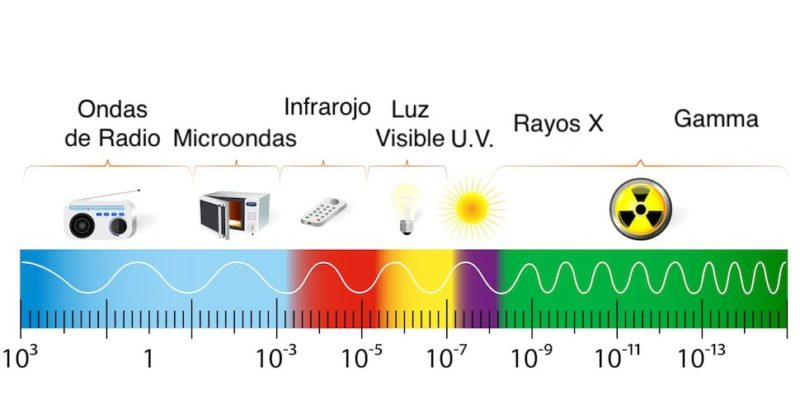
\includegraphics[width = 0.7\textwidth]{espectro}
    \caption{Representación gráfica del espectro electromagnético.}
    \label{fig:espectro}
\end{figure}

Como podemos apreciar en la figura \ref{fig:espectro} la luz es mucho más que lo vemos, se encuentra en los rayos x o gamma pasando por los microondas o las ondas de radio.

Usaremos los conceptos de frecuencia y longitud de onda de un microondas para poder medir la velocidad de la luz.


\section{Fundamento Teórico}

Como sabemos, la luz es una onda electromagnética, y como tal cumple todas las leyes por las que se rigen las ondas. Una de la más importante es:

\begin{equation}\label{eq:vel}
    v = \lambda f,
\end{equation}

donde v es la velocidad de la onda, que en este caso es lo que queremos encontrar, $\lambda$ es la longitud de onda y f la frecuencia.\cite{Laguna2010}

La longitud de onda es la distancia que hay entre dos crestas de la onda consecutivas, se ve muy claro en la imagen \ref{fig:onda}. \cite{Marion1989}

\begin{figure}[H]
    \centering
    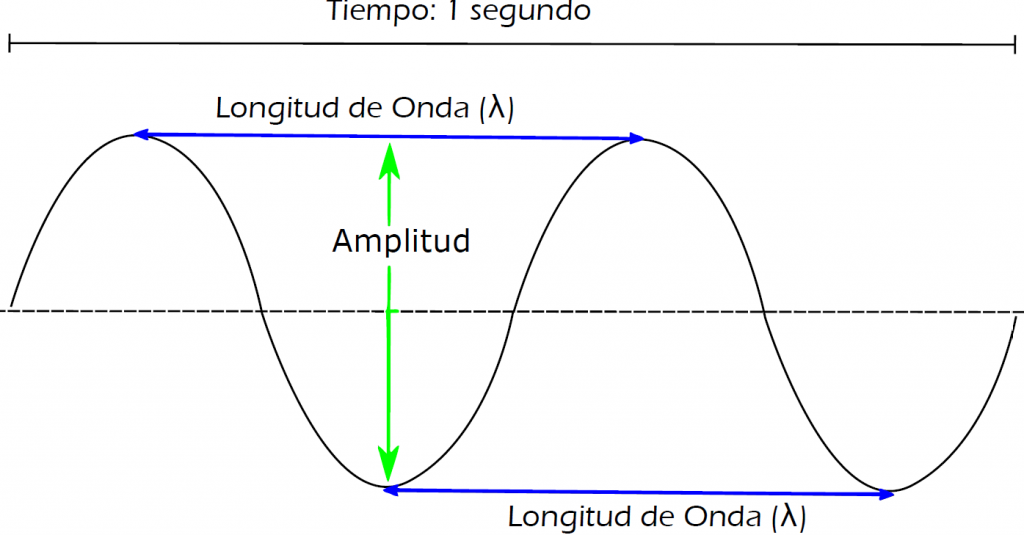
\includegraphics[width = 0.5\textwidth]{onda}
    \caption{Caption}
    \label{fig:onda}
\end{figure}

\section{Materiales y metodología}
Para realizar este experimento lo único que necesitamos es un microondas y un tranchete de queso.

Mirando el manual del microondas podremos saber la frecuencia a la que emite dicho aparato.

Ahora si metemos un tranchete en el microondas una vez quitada la pieza giratoria, veremos que el tranchete queda derretido en unas franjas y en otras no. Estas franjas corresponden con la cresta de la onda, así midiendo la distancia entre dos crestas consecutivas podremos obtener el valor de la longitud de onda, y usando la ecuación (\ref{eq:vel}) obtener la velocidad de la luz.\cite{Laguna2010}

Para este experimento usaremos un microondas nevir n-20.

\section{Resultados y conclusión}
Bien, hemos tomado los siguientes datos:  

\begin{minipage}{0.5\linewidth}
\begin{tabular}{c|c}
    \multicolumn{1}{c}{Primer set de medidas}&   \\ \hline
     Longitud de onda (m) & Error (m)\\ \hline
     0.121 & 0.004 \\ \hline
     0.120 & 0.003 \\ \hline
\end{tabular}
\end{minipage}
\begin{minipage}{0.5\linewidth}
\begin{tabular}{c|c}
    \multicolumn{1}{c}{Segundo set de medidas}&   \\ \hline
     Longitud de onda(m) & Error(m) \\ \hline 
     0.122 & 0.005 \\ \hline
     0.123 & 0.002 \\ \hline
\end{tabular}
\end{minipage}

Así que usando la fórmula (\ref{eq:vel}) llegamos a que 

$$v = 299792450 \pm 400$$.

\textit{(Para más información sobre el tratamiento de errores ver anexo)}

\section{Anexo}
Para el tratamiento de errores hemos usado la fórmula de propagación, que en este caso se quedaría:

\[\begin{array}{cc}
    \Delta v =& \sqrt{\left(\frac{\partial (\lambda f)}{\partial \lambda}\right)^2\left(\Delta\lambda\right)^2+ \left(\frac{\partial (\lambda f)}{\partial f}\right)^2 \left(\Delta f \right)^2}  \\ \\
    \Delta v =&  \sqrt{f^2(\Delta \lambda)^2 + \lambda^2 (\Delta f)^2}
\end{array}\]
\bibliography{bibli}
\end{document}
